\documentclass[border=10pt]{standalone}
\usepackage{tikz}
\usetikzlibrary{automata, positioning, arrows.meta}

\begin{document}
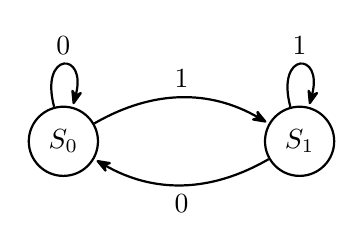
\begin{tikzpicture}[shorten >=1pt, node distance=3cm, on grid, auto, >={Stealth[round]}, thick]
    % Nodes
    \node[state] (s0) {$S_0$};
    \node[state] (s1) [right=of s0] {$S_1$};

    % Transitions
    \path[->]
        (s0) edge [loop above] node {0} (s0)
             edge [bend left] node {1} (s1)
        (s1) edge [bend left] node {0} (s0)
             edge [loop above] node {1} (s1);
\end{tikzpicture}
\end{document}
